\begin{frame}{How Many Electrons are Needed?}
  The venerable \alert<2->{Rose Criterion}\footcite{Rose_1948} provides a guideline.
  \vfill
  \uncover<2->{
    \begin{block}{The Rose Criterion}
      For proper gray-scaling, 100 electrons are needed for each pixel in the detector.
    \end{block}
  }
  \vfill
  \begin{itemize}
    \item<3-> Imaging: Single-Shot (1k x 1k detector) $\rightarrow 10^8$ electrons
    \item<4-> Imaging: Stroboscopic same but over multiple shots
    \item<5-> Diffraction: (either mode) $\rightarrow \sim10^6$ electrons
  \end{itemize}
\end{frame}

\begin{frame}{Rose Criterion Demonstrated}
\begin{figure}
  \centering
  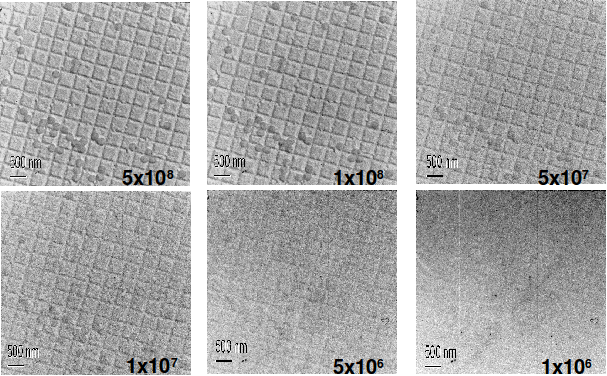
\includegraphics{ucdavis_resolution}
  \caption{From our collaborators at UCDavis / LLNL}
\end{figure}
\end{frame}

\begin{frame}{Short-pulse Child-Langmuir Law}
  \begin{itemize}
    \item Child-Langmuir Law: steady-state current limit in an electron gun
    \item Short-pulse analog: limits number of charges / area
  \end{itemize}
  \begin{columns}
    \begin{column}{0.49\linewidth}
      \begin{tikzpicture}
        \filldraw
          [fill=black!50]
          (0,0) 
            node [name=photocathode1,below right]{}
          -- ++(1,0) node [above,midway] {-V}
          -- ++(0,-5)
            node [name=source,midway] {} 
          -- ++(-1,0)
          -- cycle
        ;
        \draw
          [dashed]
          (5,0) node (ground label) [above] {Ground}
          -- ++(0,-5)
        ;
        \node [left = 0.8cm of ground label,green] {$\vec{\text{E}}$};
        \only<1-2> {
          \foreach \x in {0,...,10}
            \draw [latex-,green] (1,-\x/2) -- ++(4,0);
        }
        \only<2> {
          \draw 
            [fill=blue!10]
            (2.0,-2.5)
            ellipse (0.3 and 2.5)
          ;
        }
        \only<3> {
          \foreach \x in {0,...,5}
            \draw [latex-,green] (1,-\x) -- ++(4,0);
          \foreach \x in {1,...,5}
            \draw [latex-,green] (2.3,0.5-\x) -- ++(2.7,0);
          \draw 
            [fill=blue!40]
            (2,-2.5)
            ellipse (0.3 and 2.5)
          ;
        }
        \only<4> {
          \foreach \x in {0,...,10}
            \draw [latex-,green] (2.3,-\x/2) -- ++(2.7,0);
          \draw 
            [fill=blue!80]
            (2,-2.5)
            ellipse (0.3 and 2.5)
          ;
        }
        \only <2-> {
          \node at (2,-2.5) {$\sigma$};
          \draw 
            [-latex,very thick] 
            (2.3,-2.25) 
            -- ++(0.5,0) 
              node [above] { $ \vec{v} $ }
          ;
        }
      \end{tikzpicture}
    \end{column}
    \begin{column}{0.49\linewidth}
      \begin{itemize}
        \item<2-> For low carrier density the electric field is unaffected
        \item<3-> For higher densities ($ \sigma / \epsilon_{0} \lesssim \text{E} $) the pulse begins to screen the photocathode
        \item<4-> For limiting densities ($ \sigma / \epsilon_{0} = \text{E} $) the pulse completely screens the photocathode stopping or distorting emission
      \end{itemize}
    \end{column}
  \end{columns}
\end{frame}

\begin{frame}{Aside: UEM vs. DTEM}
Definitions: \hfill (where TOF in photogun, $t_{gun} = \sqrt{ \frac{2 m d}{q E_{DC} } } \approx$ 0.1--1ns)
\vfill
  \begin{columns}
    \begin{column}{0.49\linewidth}
      \begin{block}{Ultrafast EM (UEM)}
      \centering
      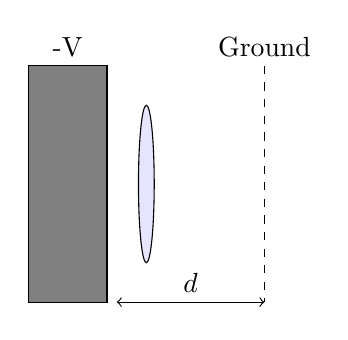
\begin{tikzpicture}
        \filldraw
          [fill=black!50]
          (0,0) 
            node [name=photocathode1,below right]{}
          -- ++(1,0) node [above,midway] {-V}
          -- ++(0,-3)
            node [name=source,midway] {} 
            node [name=bottom,pos=1] {}
          -- ++(-1,0)
          -- cycle
        ;
        \draw
          [dashed]
          (3,0) node (ground label) [above] {Ground}
          -- ++(0,-3)
        ;
        \draw 
          [fill=blue!10]
          (1.5,-1.5)
          ellipse (0.1 and 1)
        ;
        \draw [<->]
          (bottom)
          -- (bottom -| ground label)
            node [pos=0.5,above] {$d$}
        ;
      \end{tikzpicture}\\
      Short-pulse Child's Law applies\\
      $\tau_{pulse} < t_{gun}$
      \end{block}
    \end{column}
    \begin{column}{0.49\linewidth}
      \begin{block}{Dynamic TEM (DTEM)}
      \centering
      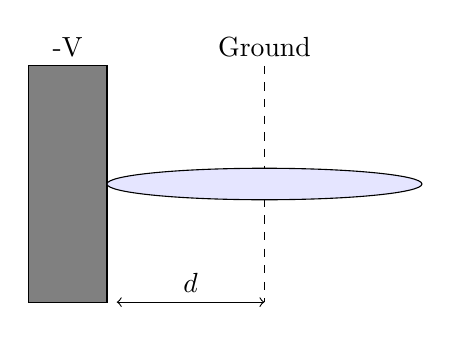
\begin{tikzpicture}
        \filldraw
          [fill=black!50]
          (0,0) 
            node [name=photocathode1,below right]{}
          -- ++(1,0) node [above,midway] {-V}
          -- ++(0,-3)
            node [name=source,midway] {}
            node [name=bottom,pos=1] {}
          -- ++(-1,0)
          -- cycle
        ;
        \draw
          [dashed]
          (3,0) node (ground label) [above] {Ground}
          -- ++(0,-3)
        ;
        \draw 
          [fill=blue!10]
          (3,-1.5)
          ellipse (2 and 0.2)
        ;
        \draw [<->]
          (bottom)
          -- (bottom -| ground label)
            node [pos=0.5,above] {$d$}
        ;
      \end{tikzpicture}\\
      Child-Langmuir Law applies\\
      $\tau_{pulse} > t_{gun}$
      \end{block}
    \end{column}
  \end{columns}
\end{frame}

\begin{frame}{Aside: UEM vs. DTEM}
\begin{center}
\begin{tikzpicture}
  \node (image) {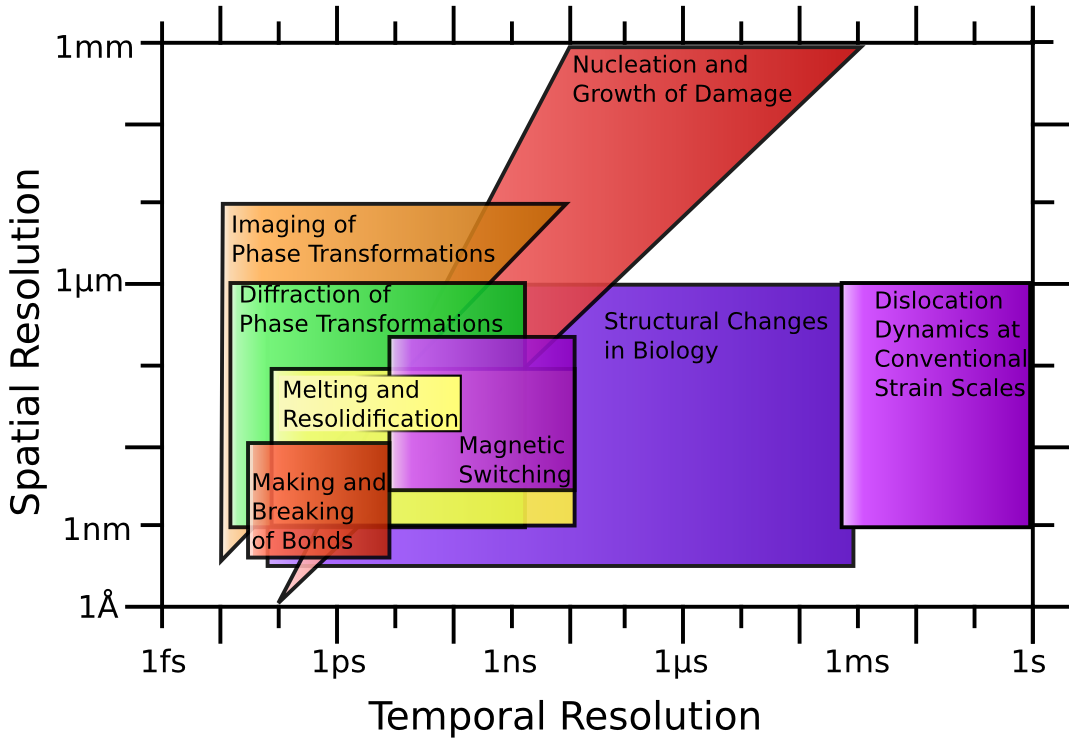
\includegraphics[width=0.7\linewidth]{Resolution}};
  \visible<2->{
    \node [
      star,
      star point ratio = 2,
      inner sep = 0.7mm,
      draw,
      fill=white,
      pin={[draw,fill=white,pin edge=thick] above:{\tiny TU-Berlin}}
    ] at (0.3,0.1) {};
    \node [
      star,
      star point ratio = 2,
      inner sep = 0.7mm,
      draw,
      fill=white,
      pin={[draw,fill=white,pin edge=thick] right:{\tiny UEM-2 Caltech}}
    ] at (0.3,-0.3) {};
    \node [
      star,
      star point ratio = 2,
      inner sep = 0.7mm,
      draw,
      fill=white,
      pin={[draw,fill=white,pin edge=thick,pin distance=0.6in] above:{\tiny Caltech stroboscopic}}
    ] at (-1.3,-0.3) {};
    \node [
      star,
      star point ratio = 2,
      inner sep = 0.7mm,
      draw,
      fill=white,
      pin={[draw,fill=white,pin edge=thick] right:{\tiny LLNL}}
    ] at (0.4,-0.6) {};
    \node [
      star,
      star point ratio = 2,
      inner sep = 0.7mm,
      draw,
      fill=white,
      pin={[draw,fill=white,pin edge=thick] right:{\tiny UC-Davis Bio-DTEM}}
    ] at (1.2,-1.1) {};
  }
  \visible<3->{
    \node[above=0.5mm of image] (text) {TOF in photogun, $t_{gun} = \sqrt{ \frac{2 m d}{q E_{DC} } } \approx$ 0.1--1ns};
  }
  \visible<4->{
    \draw<3->[fill=red!20,opacity=0.9] (-0.64,-1.85) rectangle (-0.17,2.56) node[left=0.1] (box) {};
    \draw<3->[->,thick,red] 
      (text.350) 
        to [out=-110,in=70] (box)
    %-- (box)
    ;
  }
  \visible<5->{
    \node [red] at (-2,2.2) {UEM};
    \node [red] at (3,2.2) {DTEM};
  }
\end{tikzpicture}
\end{center}
\end{frame}

\begin{frame}{Implications of SPCL for TR-EM}
  The results of the previous concepts lead to a simple conclusion:
  \vfill
  \begin{block}{}
  \begin{figure}
    \centering
    \begin{tikzpicture} [every node/.style={draw,fill=white,text badly centered,text width=3cm}]
      \node (charges)  {Need a high number of charges};
      \node (child) [below=0.5cm of charges] {Child's law limits charges per area};
      \node (result1) at ($(charges)!0.5!(child) + (4,0)$) {Need a large emission area};
      
      \draw [-latex] (charges) -- (result1);
      \draw [-latex] (child) -- (result1);
    \end{tikzpicture}
  \end{figure}
  \end{block}
  \vfill
  \uncover<2->{Further, large beam width necessitates custom, large bore TEM hardware}
\end{frame}

